% Standalone version of Figure 1: Tree of Knowledge
% Compile with: pdflatex figure1-standalone.tex
\documentclass[border=10pt]{standalone}
\usepackage{tikz}
\usetikzlibrary{arrows.meta}
\usepackage[T1]{fontenc}
\usepackage{helvet}
\renewcommand{\familydefault}{\sfdefault}

\begin{document}
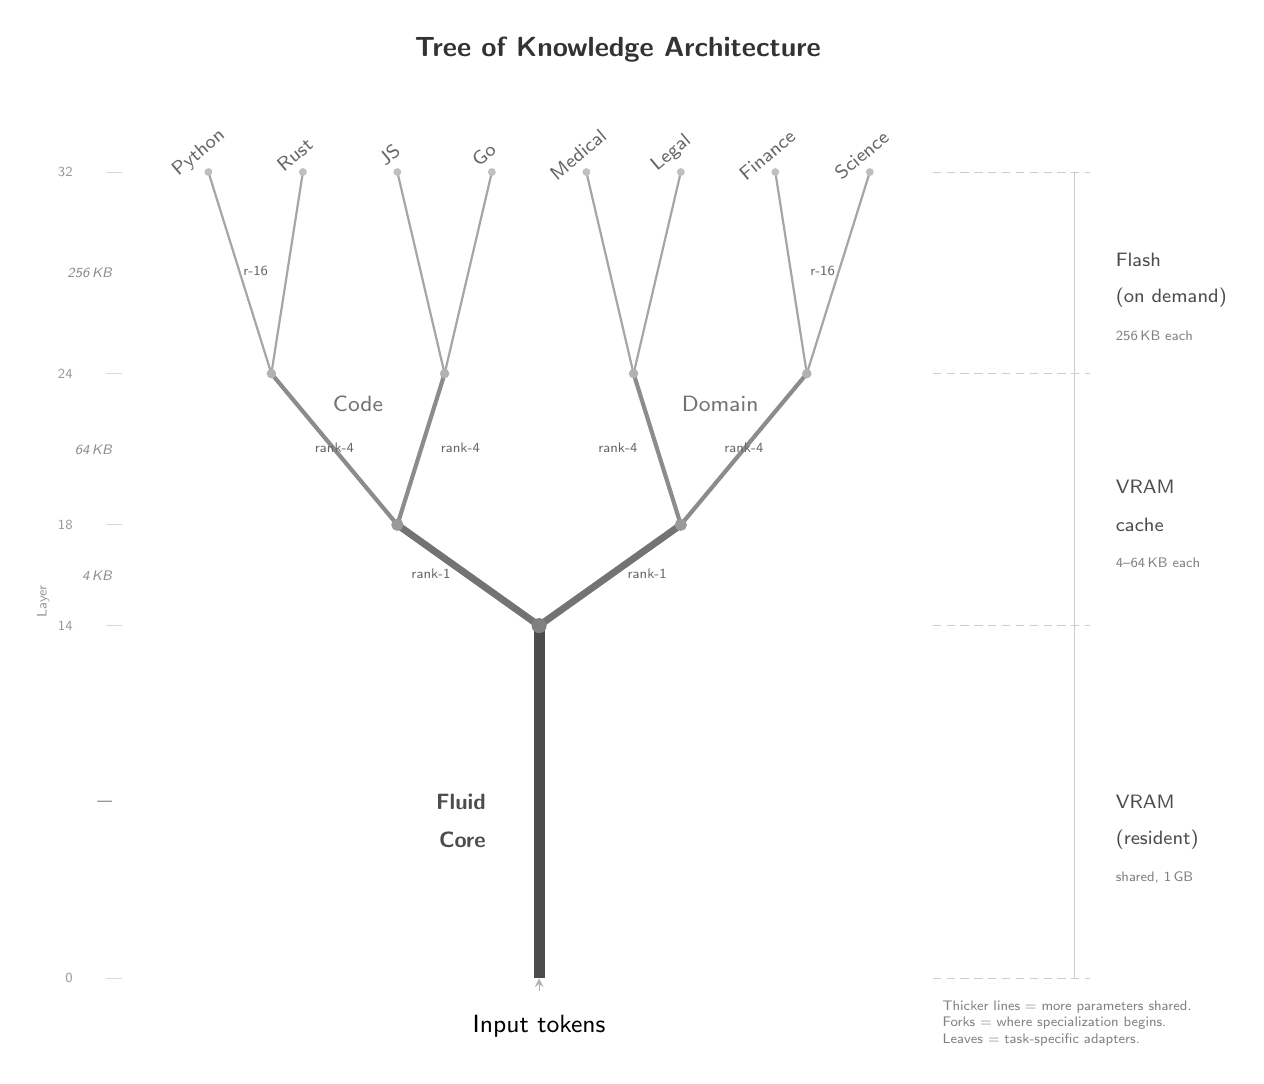
\begin{tikzpicture}[
    x=1cm, y=0.32cm,
    trunk/.style={line width=4pt, color=black!70},
    branch2/.style={line width=2.5pt, color=black!55},
    branch4/.style={line width=1.5pt, color=black!45},
    branch8/.style={line width=0.8pt, color=black!35},
    nodelabel/.style={font=\sffamily\scriptsize, inner sep=2pt},
    ranklabel/.style={font=\sffamily\tiny, color=black!60},
    tierlabel/.style={font=\sffamily\small, anchor=west, text=black!70},
    tierbox/.style={draw=none, rounded corners=1pt, inner sep=3pt},
    layermark/.style={font=\sffamily\tiny, color=black!40, anchor=east},
]

% === Coordinates ===
% Vertical: layers 0 (input) to 32 (output)
% Horizontal: centered at 0, branches spread outward

% --- Layer tick marks (left side) ---
\foreach \y/\lbl in {0/0, 14/14, 18/18, 24/24, 32/32} {
    \node[layermark] at (-5.8, \y) {\lbl};
    \draw[black!15, thin] (-5.5, \y) -- (-5.3, \y);
}
\node[font=\sffamily\tiny, color=black!40, anchor=east, rotate=90] at (-6.3, 16) {Layer};

% --- Trunk: layers 0--14 ---
\draw[trunk] (0, 0) -- (0, 14);

% Input token marker
\node[nodelabel, anchor=north, font=\sffamily\small] at (0, -1.2) {Input tokens};
\draw[black!30, thin, -{stealth}] (0, -0.5) -- (0, 0);

% Trunk label
\node[nodelabel, anchor=east, font=\sffamily\footnotesize\bfseries, text=black!70] at (-0.6, 7) {Fluid};
\node[nodelabel, anchor=east, font=\sffamily\footnotesize\bfseries, text=black!70] at (-0.6, 5.5) {Core};

% --- First fork: layer 14 → 18, into 2 branches ---
\draw[branch2] (0, 14) -- (-1.8, 18);
\draw[branch2] (0, 14) -- (1.8, 18);

% Fork node
\filldraw[black!50] (0, 14) circle (2.5pt);

% Rank labels at first fork
\node[ranklabel, anchor=south east] at (-1.0, 15.5) {rank-1};
\node[ranklabel, anchor=south west] at (1.0, 15.5) {rank-1};

% --- Second fork: layer 18 → 24, each into 2 (total 4) ---
% Left branch splits
\draw[branch4] (-1.8, 18) -- (-3.4, 24);
\draw[branch4] (-1.8, 18) -- (-1.2, 24);
\filldraw[black!40] (-1.8, 18) circle (2pt);

% Right branch splits
\draw[branch4] (1.8, 18) -- (1.2, 24);
\draw[branch4] (1.8, 18) -- (3.4, 24);
\filldraw[black!40] (1.8, 18) circle (2pt);

% Rank labels at second fork
\node[ranklabel, anchor=south] at (-2.6, 20.5) {rank-4};
\node[ranklabel, anchor=south] at (-1.0, 20.5) {rank-4};
\node[ranklabel, anchor=south] at (1.0, 20.5) {rank-4};
\node[ranklabel, anchor=south] at (2.6, 20.5) {rank-4};

% --- Third fork: layer 24 → 32, each into 2 (total 8) ---
% From -3.4
\draw[branch8] (-3.4, 24) -- (-4.2, 32);
\draw[branch8] (-3.4, 24) -- (-3.0, 32);
\filldraw[black!30] (-3.4, 24) circle (1.5pt);

% From -1.2
\draw[branch8] (-1.2, 24) -- (-1.8, 32);
\draw[branch8] (-1.2, 24) -- (-0.6, 32);
\filldraw[black!30] (-1.2, 24) circle (1.5pt);

% From 1.2
\draw[branch8] (1.2, 24) -- (0.6, 32);
\draw[branch8] (1.2, 24) -- (1.8, 32);
\filldraw[black!30] (1.2, 24) circle (1.5pt);

% From 3.4
\draw[branch8] (3.4, 24) -- (3.0, 32);
\draw[branch8] (3.4, 24) -- (4.2, 32);
\filldraw[black!30] (3.4, 24) circle (1.5pt);

% Rank labels at third fork
\node[ranklabel, anchor=south] at (-3.6, 27.5) {r-16};
\node[ranklabel, anchor=south] at (3.6, 27.5) {r-16};

% --- Leaf labels (specializations) ---
\node[nodelabel, anchor=south, rotate=40, text=black!60] at (-4.2, 32.3) {Python};
\node[nodelabel, anchor=south, rotate=40, text=black!60] at (-3.0, 32.3) {Rust};
\node[nodelabel, anchor=south, rotate=40, text=black!60] at (-1.8, 32.3) {JS};
\node[nodelabel, anchor=south, rotate=40, text=black!60] at (-0.6, 32.3) {Go};
\node[nodelabel, anchor=south, rotate=40, text=black!60] at (0.6, 32.3) {Medical};
\node[nodelabel, anchor=south, rotate=40, text=black!60] at (1.8, 32.3) {Legal};
\node[nodelabel, anchor=south, rotate=40, text=black!60] at (3.0, 32.3) {Finance};
\node[nodelabel, anchor=south, rotate=40, text=black!60] at (4.2, 32.3) {Science};

% Leaf dots
\foreach \x in {-4.2, -3.0, -1.8, -0.6, 0.6, 1.8, 3.0, 4.2} {
    \filldraw[black!25] (\x, 32) circle (1.2pt);
}

% --- Branch group labels (mid-level) ---
\node[nodelabel, font=\sffamily\footnotesize, text=black!55] at (-2.3, 22.8) {Code};
\node[nodelabel, font=\sffamily\footnotesize, text=black!55] at (2.3, 22.8) {Domain};

% === Right-side storage tier annotations ===
% Use dashed horizontal lines and labels

% Tier 1: VRAM resident (trunk)
\draw[black!20, densely dashed] (5.0, 0) -- (7.0, 0);
\draw[black!20, densely dashed] (5.0, 14) -- (7.0, 14);
\draw[black!20, thin] (6.8, 0) -- (6.8, 14);
\node[tierlabel, font=\sffamily\scriptsize] at (7.2, 7) {VRAM};
\node[tierlabel, font=\sffamily\scriptsize] at (7.2, 5.5) {(resident)};
\node[tierlabel, font=\sffamily\tiny, text=black!50] at (7.2, 4) {shared, 1\,GB};

% Tier 2: VRAM cache (shallow branches)
\draw[black!20, densely dashed] (5.0, 14) -- (7.0, 14);
\draw[black!20, densely dashed] (5.0, 24) -- (7.0, 24);
\draw[black!20, thin] (6.8, 14) -- (6.8, 24);
\node[tierlabel, font=\sffamily\scriptsize] at (7.2, 19.5) {VRAM};
\node[tierlabel, font=\sffamily\scriptsize] at (7.2, 18) {cache};
\node[tierlabel, font=\sffamily\tiny, text=black!50] at (7.2, 16.5) {4--64\,KB each};

% Tier 3: Flash storage (deep branches)
\draw[black!20, densely dashed] (5.0, 24) -- (7.0, 24);
\draw[black!20, densely dashed] (5.0, 32) -- (7.0, 32);
\draw[black!20, thin] (6.8, 24) -- (6.8, 32);
\node[tierlabel, font=\sffamily\scriptsize] at (7.2, 28.5) {Flash};
\node[tierlabel, font=\sffamily\scriptsize] at (7.2, 27) {(on demand)};
\node[tierlabel, font=\sffamily\tiny, text=black!50] at (7.2, 25.5) {256\,KB each};

% === Size annotations along left side ===
\node[ranklabel, anchor=east] at (-5.3, 7) {---};
\node[ranklabel, anchor=east, font=\sffamily\tiny\itshape, text=black!45] at (-5.3, 16) {4\,KB};
\node[ranklabel, anchor=east, font=\sffamily\tiny\itshape, text=black!45] at (-5.3, 21) {64\,KB};
\node[ranklabel, anchor=east, font=\sffamily\tiny\itshape, text=black!45] at (-5.3, 28) {256\,KB};

% === Bottom-right: concise key ===
\node[anchor=north west, font=\sffamily\tiny, text=black!50, text width=3.5cm] at (5.0, -0.5) {
    Thicker lines = more parameters shared.\\
    Forks = where specialization begins.\\
    Leaves = task-specific adapters.
};

% === Title (standalone only) ===
\node[anchor=south, font=\sffamily\normalsize\bfseries, text=black!80] at (1, 36) {Tree of Knowledge Architecture};

\end{tikzpicture}
\end{document}
